\documentclass[letterpaper, 10 pt, conference]{ieeeconf}

\IEEEoverridecommandlockouts
\overrideIEEEmargins

\usepackage{graphicx}
\usepackage{caption}

\title{\LARGE \bf
General CRF Classifiers for Temporal Expression and Event Extraction: \\ An Experimental Approach
}

\author{
  Israney, Ankush\\
  Drexel University
  \and
  Ramakrishna, Jaidev\\
  Drexel University
}

\begin{document}

\maketitle
\thispagestyle{empty}
\pagestyle{empty}

\begin{abstract}
In the past decade, advances in Machine Learning techniques have led to significant improvements in the recognition subtask of the Named Entity Recognition Problem. Systems deploying Machine Learning techniques show great promise in the NER problem of Natural Language Processing because they reduce significant human effort to annotate vast amounts of information.

This paper describes existing methodology we have used to perform extraction of Temporal Expressions and Events from text obtained from the News domain using Conditional Random Fields, describes the architecture of the system we have built for this task, and systematically analyzes the results we have obtained. Following the suggestion by Str¨otgen and Gertz\cite{c7}, we also compare our results to recent research conducted using general CRF classifiers used in the clinical domain.

\end{abstract}

\section{INTRODUCTION}

Natural Language Processing is still an open problem and an active area of Research. Recent efforts focus on the integration of Machine Learning algorithms to solve NLP tasks, and hence reduce human effort. Named Entity Recognition is a subtask in Information Retrieval that is concerned with identifying entities in pieces of arbitrary raw text. These entities can be Persons, Organizations, Places, Times, Events etc.  Another important facet of the NER task is normalization - identifying and unifying multiple Temporal expressions that refer to or are concerned with the same value.

A Temporal expression is any expression that encodes or expresses information pertaining to time. These expressions may be of several types - implicit (eg. a festival or holiday which are to be inferred), explicit/absolute (an explicit date or time), or relative (w.r.t some other expression in the document or with the document creation time).

Furthermore, it is useful to link these expressions to other events and the temporal expressions that they are concerned with. These relations can be used in other research problems, like Conversion to Logic forms and Causality, to name a few. Conditlional Random Fields are especially suited to this task since they are able to recognize and encode context for sequnetial classification of labels\cite{c6}.
\section{Task Description}

The TempEval task is a temporal annotation task conducted as part of the SemEval competition series to annotate time and event expressions. The task initially comprised of identifying relations between temporal expressions, but with evolving annotations used to annotate temporal expressions, TempEval in the Named Entity Recognition task is composed of 6 subtasks: TS, to identify the span of temporal expressions, 
ES - to identify span of events, EA - to identify attributes of event expressions, TA - to identify attributes of time expressions, DR - to identify relations between events and the document creation time and CR - to identify container relations (expressions contained within each other). In this paper, we focus on the the identification tasks (TS and ES) and perform  an in-depth experimental evaluation of the results of the general CRF classifiers used in these tasks. 

Our Training dataset consists of 2452 news transcripts obtained from the tempEval-3 task\footnote[1]{https://www.cs.york.ac.uk/semeval-2013/task1/index.php}, which are used for training our model using the Stanford-NER CRF classifier. Our testing set is a manually annotated dataset from the tempEval-3 task along with the expected tags annotated in the TimeML specification language. The dataset is a subset of the original TimeBank news corpora used in the competition. TimeML is a specification language to annotate events and temporal expressions in a hierarchy using xml as an underlying framework.

\section{RECOGNITION TASK}

The respective Span Identification sub-tasks of the TempEval series are the only tasks which have consistently proven to perform better than existing rule-based methods. Most existing work in the community follow a hybrid approach to perform identification using existing ML techniques, and use rule-based methods for assigning values to attributes of these expressions (specifically for normalization to assign values to these identified instances). For instance, 26th November 2016, 11/26/2016 and Thanksgiving '16 all refer to the same date in time normalized form, which refer 26-11-2016. The community considers this task conducive to thousands of manually constructed rules rather than automatic assignment using even the most recent advances in ML techniques. In this paper we focus on the identification tasks without normalization to study the effects of the Training set size on task performance, discuss a qualitative approach to analyze performance, and compare the results of Conditional Random Fields in our chosen News domain to other instances of recent research in the Clinical domain deploying similar techniques.

\section{METHODOLOGY}

\subsection{Conditional Random Fields}

Conditional Random Fields have gained significant popularity in the NER branch of NLP tasks over the past decade. Sutton and McCallum\cite{c6} suggest that CRF's combine the ability of graphical models which model multivariate data in a compact manner and the ability of classification models which use large sets of input features to perform predictions. These models provide for structured prediction in sequential applications than most of their generative counterparts. This notion is fundamental to numerous applications where variables have known to have conditional dependency upon each other.

Hidden Markov Models, which are generative models, make 2 assumptions which conflict with our goals for the NER task \cite{c6}. Firstly, it assumes that each state only depends on its immediate predecessor. Secondly, each observation variable depends on only the current state. Therefore, when an HMM is deployed in the NER task, it utilizes the initial distribution, the transition distribution and the emission (observation)\cite{c6}. If entities like temporal expressions occur sparsely in the training set, this would render the word (as a feature) uninformative. Therefore, we need to exploit other features of the word, its neighboring words, prefixes and suffixes, and n-grams, and weight them conditionally.

In contrast, CRF's exploit the concept of feature functions, where each feature has the form $$f_{k}(y, y_{y-1}, x_t) $$ 

There is 1 feature for each transition and 1 feature for each state-observation pair. The conditional distribution which results from this HMM like form is a linear-CRF:
$$
p(y, x) = \frac{1}{Z}\prod_{t=1}^Texp(\sum_{k=1}^{K}\theta_kf_k(y_t, y_{t-1}, x_t))
$$

This linear CRF is the basic form of the Stanford NER general CRF used in the NER task - 
$$
p(y, x) = \frac{1}{Z(x)}\prod_{t=1}^Texp(\sum_{k=1}^{K}\theta_{ak}f_{ak}(y_a, x_a))
$$

Conditioning simplifies the graphical model where Z(x) is computable instead of Z in the linear CRF case. The formal definition is: \\

"Let $G$ be a factor graph over $X$ and $Y$. Then $(X, Y)$ is a conditional random field if for any value x of $X$, the distribution factorizes according to G." \cite{c6} 

\subsection{Input Features}
Theses are the features that we are using in our system. The following descriptions are quoted from the documentation of the NERFeatureFactory class in the CRFClassifier documentation.\cite{c12}
\begin{itemize}
\item \textbf{useClassFeature} - Include a feature for the class (as a class marginal). Puts a prior on the classes which is equivalent to how often the feature appeared in the training data.
\item \textbf{useWord} - Gives Feature for w
\item \textbf{useNGrams} - Make features from letter n-grams, i.e., substrings of the word
\item \textbf{noMidNGrams} - Do not include character n-gram features for n-grams that contain neither the beginning or end of the word
\item \textbf{maxNGramLeng} - If this number is positive, n-grams above this size will not be used in the model
\item \textbf{usePrev} - Gives you feature for (pw,c), and together with other options enables other previous features, such as (pt,c)
\item \textbf{useNext} - Gives you feature for (nw,c), and together with other options enables other next features, such as (nt,c)
\item \textbf{useDisjunctive} - Include in features giving disjunctions of words anywhere in the left or right disjunctionWidth words (preserving direction but not position)
\item \textbf{useSequences} - Does not use any class combination features if this is false
\item \textbf{usePrevSequences} - Does not use any class combination features using previous classes if this is false
\item \textbf{useTypeSeqs} - Use basic zeroeth order word shape features.
\item \textbf{useTypeSeqs2} - Add additional first and second order word shape features
\item \textbf{useTypeySequences} - Some first order word shape patterns.
\item \textbf{wordShape} - Either "none" for no wordShape use, or the name of a word shape function.
\end{itemize}

\section{IMPLEMENTATION DETAILS}

The system we have built utilizes two powerful and popular open source NLP systems, along with our own code to integrate them.

\subsection{CoreNLP}
This is a suite of NLP tools written in Java, developed at Stanford university\cite{c3}. Its main use is as a tagger for Parts of Speech. Not only is it capable of identifying which parts of speech words fall into, but also of recognizing and encoding relationships between them. It supports multiple human languages, and has wrappers and bindings for various programming languages. In our system, we use CoreNLP for preprocessing our training set.


\subsection{Stanford NER}
Stanford NER is a Named Entity Recognizer implemented in Java that is used to label entities with their types, like Person, Event, Time etc \cite{c4}. It has also been adapted for other tasks like Protein and Gene tagging. This is the core of our system - specifically, the CRFClassifier class. We use it to produce our model using the training files, and then to test the model using the testing files. We can specify the features to be extracted using a properties file, and can fine tune the execution using command line arguments.

\subsection{Integration Code}
Various classes of the above mentioned packages have very specific requirements for their input files. Specifically, the TimeML and TSV formats are used. Elsewhere, they required plain text files. Hence, it was necessary for us to write preprocessors and converters to produce the correct formats. We obtained one particular converter that accepted TimeML files and converted them to COL files from an open source project\footnote[2]{https://github.com/paramitamirza/TimeML-CAT-Converter}.

\section{EXPERIMENTAL SETUP \& RESULTS}
Our project has been created to run on Ubuntu Linux, but we anticipate no problems if it is run on any reasonably modern Linux, or indeed any POSIX compliant system.

Both of the NLP systems mentioned above are written in Java. The code we produced is in Python, and hence we have used Python bindings and wrappers for both systems. Therefore, Java 8+ and Python 2.7+ will be necessary for our project to work. One should note that the specific implementations we tested on were Oracle Java 8 and CPython. We encountered some minor issues on a system running OpenJDK and Jython.

The conversion and training portions of our system are memory and processor intensive. We tested our project on a machine with 16GB of RAM and an Intel Corei7 6700HQ processor. It requires over 1 hour to complete, including training and testing. CoreNLP uses a command line argument to specify how much memory it is allowed to use. We have hard coded our project to allocate 4GB of RAM, but this can be easily modified. Nevertheless, it is inadvisable to run the code with less than 8GB of RAM.

Below are all results for precision, recall and f-measure for different sizes of Training set.

\begin{table}[!htpb]
\centering
\caption{Training Set Size = 10}
\label{t1}
\begin{tabular}{lcccccc}
\textbf{Entity} & \textbf{P} & \textbf{R} & \textbf{F1} & \textbf{TP} & \textbf{FP} & \textbf{FN} \\
\hline
\textbf{EVENT}  & 0.7929     & 0.2435     & 0.3726      & 356         & 93          & 1106        \\
\textbf{OTHERS} & 0.2202     & 0.0633     & 0.0984      & 109         & 386         & 1612        \\
\textbf{TIMEX3} & 0.875      & 0.1014     & 0.1818      & 28          & 4           & 248         \\
\textbf{Totals} & 0.5051     & 0.1425     & 0.2223      & 493         & 483         & 296        
\end{tabular}
\end{table}

\begin{table}[!htpb]
\centering
\caption{Training Set Size = 50}
\label{t2}
\begin{tabular}{lcccccc}
\textbf{Entity} & \textbf{P} & \textbf{R} & \textbf{F1} & \textbf{TP} & \textbf{FP} & \textbf{FN} \\
\hline
\textbf{EVENT}  & 0.7904     & 0.5157     & 0.6242      & 754         & 200         & 708         \\
\textbf{OTHERS} & 0.4246     & 0.2766     & 0.335       & 476         & 645         & 1245        \\
\textbf{TIMEX3} & 0.8882     & 0.5181     & 0.6545      & 143         & 18          & 133         \\
\textbf{Totals} & 0.614      & 0.3969     & 0.4822      & 1373        & 863         & 2086       
\end{tabular}
\end{table}

\begin{table}[!htpb]
\centering
\caption{Training Set Size = 100}
\label{t3}
\begin{tabular}{lcccccc}
\textbf{Entity} & \textbf{P} & \textbf{R} & \textbf{F1} & \textbf{TP} & \textbf{FP} & \textbf{FN} \\
\hline
\textbf{EVENT}  & 0.793      & 0.5923     & 0.6782      & 866         & 226         & 596         \\
\textbf{OTHERS} & 0.468      & 0.3481     & 0.3992      & 599         & 681         & 1122        \\
\textbf{TIMEX3} & 0.8866     & 0.6232     & 0.7319      & 172         & 22          & 104         \\
\textbf{Totals} & 0.638      & 0.4733     & 0.5434      & 1637        & 929         & 1822       
\end{tabular}
\end{table}

\begin{table}[!htpb]
\centering
\caption{Training Set Size = 200}
\label{t4}
\begin{tabular}{lcccccc}
\textbf{Entity} & \textbf{P} & \textbf{R} & \textbf{F1} & \textbf{TP} & \textbf{FP} & \textbf{FN} \\
\hline
\textbf{EVENT}  & 0.804      & 0.6676     & 0.7294      & 976         & 238         & 486         \\
\textbf{OTHERS} & 0.5351     & 0.4346     & 0.4796      & 748         & 650         & 973         \\
\textbf{TIMEX3} & 0.9362     & 0.6377     & 0.7586      & 176         & 12          & 100         \\
\textbf{Totals} & 0.6786     & 0.5493     & 0.6071      & 1900        & 900         & 1559       
\end{tabular}
\end{table}

\begin{table}[!htpb]
\centering
\caption{Training Set Size = 500}
\label{t5}
\begin{tabular}{lcccccc}
\textbf{Entity} & \textbf{P} & \textbf{R} & \textbf{F1} & \textbf{TP} & \textbf{FP} & \textbf{FN} \\
\hline
\textbf{EVENT}  & 0.8094     & 0.7202     & 0.7622      & 1053        & 248         & 409         \\
\textbf{OTHERS} & 0.5774     & 0.5009     & 0.5364      & 862         & 631         & 859         \\
\textbf{TIMEX3} & 0.949      & 0.6739     & 0.7881      & 186         & 10          & 90          \\
\textbf{Totals} & 0.7027     & 0.6074     & 0.6516      & 2101        & 889         & 1358       
\end{tabular}
\end{table}

\begin{table}[!htpb]
\centering
\caption{Training Set Size = 1000}
\label{t6}
\begin{tabular}{lcccccc}
\textbf{Entity} & \textbf{P} & \textbf{R} & \textbf{F1} & \textbf{TP} & \textbf{FP} & \textbf{FN} \\
\hline
\textbf{EVENT}  & 0.8144     & 0.7442     & 0.7777      & 1088        & 248         & 374         \\
\textbf{OTHERS} & 0.5944     & 0.5288     & 0.5597      & 910         & 621         & 811         \\
\textbf{TIMEX3} & 0.9261     & 0.6812     & 0.785       & 188         & 15          & 88          \\
\textbf{Totals} & 0.7121     & 0.632      & 0.6696      & 2186        & 884         & 1273       
\end{tabular}
\end{table}

\begin{table}[!htpb]
\centering
\caption{Training Set Size = 1500}
\label{t7}
\begin{tabular}{lcccccc}
\textbf{Entity} & \textbf{P} & \textbf{R} & \textbf{F1} & \textbf{TP} & \textbf{FP} & \textbf{FN} \\
\hline
\textbf{EVENT}  & 0.809      & 0.7592     & 0.7833      & 1110        & 262         & 352         \\
\textbf{OTHERS} & 0.6045     & 0.5497     & 0.5758      & 946         & 619         & 775         \\
\textbf{TIMEX3} & 0.9561     & 0.7101     & 0.815       & 196         & 9           & 80          \\
\textbf{Totals} & 0.7167     & 0.6511     & 0.6823      & 2252        & 890         & 1207       
\end{tabular}
\end{table}

\begin{table}[!htpb]
\centering
\caption{Training Set Size = 2000}
\label{t8}
\begin{tabular}{lcccccc}
\textbf{Entity} & \textbf{P} & \textbf{R} & \textbf{F1} & \textbf{TP} & \textbf{FP} & \textbf{FN} \\
\hline
\textbf{EVENT}  & 0.8067     & 0.7538     & 0.7793      & 1102        & 264         & 360         \\
\textbf{OTHERS} & 0.5959     & 0.5415     & 0.5674      & 932         & 632         & 789         \\
\textbf{TIMEX3} & 0.9429     & 0.7174     & 0.8148      & 198         & 12          & 78          \\
\textbf{Totals} & 0.7108     & 0.6453     & 0.6765      & 2232        & 908         & 1227       
\end{tabular}
\end{table}

\begin{table}[!htpb]
\centering
\caption{Training Set Size = 2452}
\label{t9}
\begin{tabular}{lcccccc}
\textbf{Entity} & \textbf{P} & \textbf{R} & \textbf{F1} & \textbf{TP} & \textbf{FP} & \textbf{FN} \\
\hline
\textbf{EVENT}  & 0.8115     & 0.7715     & 0.791       & 1128        & 262         & 334         \\
\textbf{OTHERS} & 0.5999     & 0.5532     & 0.5756      & 952         & 635         & 769         \\
\textbf{TIMEX3} & 0.9378     & 0.7101     & 0.8082      & 196         & 13          & 80          \\
\textbf{Totals} & 0.7144     & 0.658      & 0.685       & 2276        & 910         & 1183       
\end{tabular}
\end{table}

\section{QUALITATIVE ANALYSIS}

\subsection{Graphical Representation}
Below are the Graphs for True-Positives, False-Positives and False-Negatives for each of the EVENT, OTHERS and TIMEX3 expressions respectively, followed by the performance of our CRF Classifer in terms of Precision, Recall and f-measure for TIMEX3, EVENT AND OTHER CLASSES. These graphs have been created from the data in Tables I to IX. It should be noted that the OTHER class is not the same as the O class that is used by the classifier. O indicates that identification was not possible. OTHER indicates that classification was possible, but the class was neither an EVENT nor a TIMEX3.

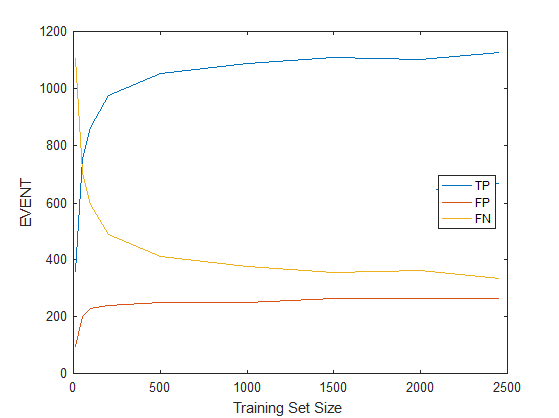
\includegraphics[scale = 0.65]{f1.png}
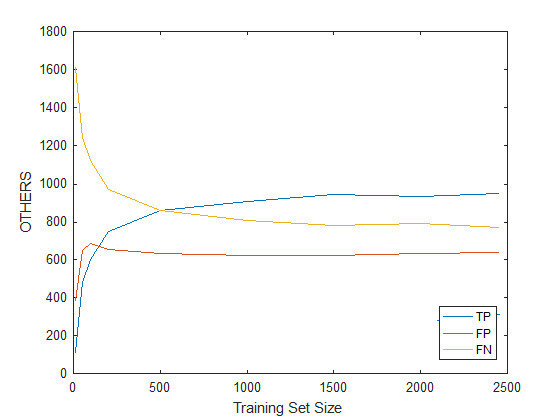
\includegraphics[scale = 0.65]{f2.png}
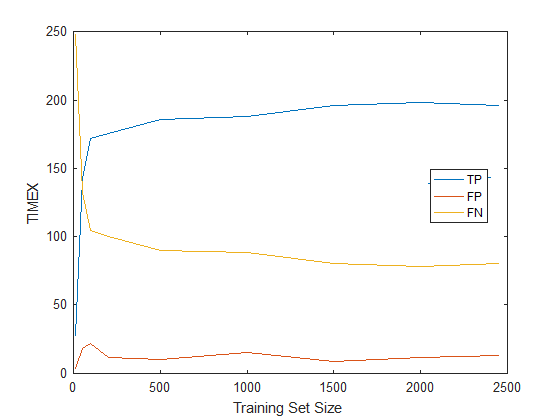
\includegraphics[scale = 0.65]{f3.png}
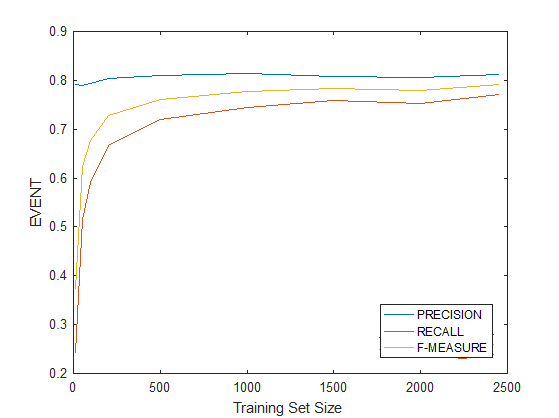
\includegraphics[scale = 0.65]{f4.png}
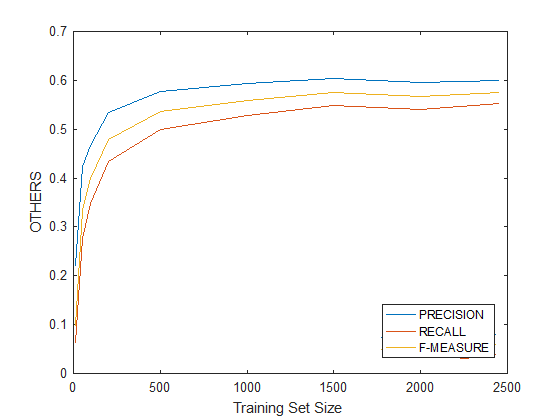
\includegraphics[scale = 0.65]{f5.png}
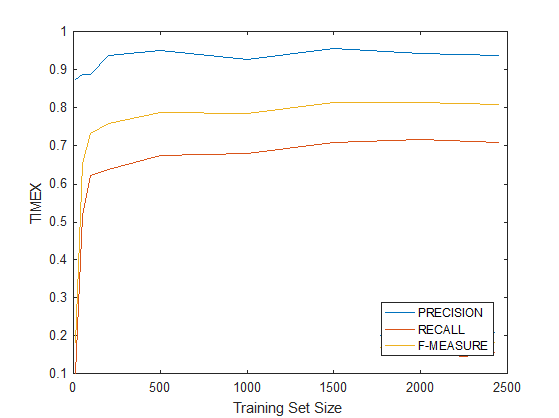
\includegraphics[scale = 0.65]{f6.png}

\addtolength{\textheight}{-0cm}

As seen above from the graphs, the True positives and False negatives for all classes are identical mirror images of each other, and after an initial increase/decrease period they continue to stabilize along a logarithmic trend. The False positives also decrease, but the change is too small to be seen clearly on this graph scale. This reveals the important finding that the system is trying to increase its True Positives and thereby reduce the from the False Negatives, but only manages to reduce its own False Positives very slowly. \\

Our Claims easily fit into our graphs for precision, recall and f-measure as well since Recall and f-measure following the TP and FN show a very slow but visible logarithmic increase but precision (except for the OTHERS class initially) remains almost invariant since TP increases and FP does not keep up to this growth.

\subsection{Comparison to Results from Clinical Domain}

\begin{table}[!htpb]
\centering
\caption{Events\cite{c1}}
\label{t10}
\begin{tabular}{lcccccc}
\textbf{Events}   & \textbf{P} & \textbf{R} & \textbf{F}\\
\hline
\textbf{Clinical} & 0.835      & 0.797      & 0.815\\
\textbf{Ours}     & 0.8115     & 0.7715     & 0.7910\\
\end{tabular}
\end{table}

\begin{table}[!htpb]
\centering
\caption{TimeX3\cite{c2}}
\label{t11}
\begin{tabular}{lcccccc}
\textbf{TimeX3}   & \textbf{P} & \textbf{R} & \textbf{F}\\
\hline
\textbf{Clinical} & 0.821      & 0.669      & 0.737\\
\textbf{Ours}     & 0.9378     & 0.7101     & 0.8082\\
\end{tabular}
\end{table}



In tables X and XI, we compare our work to the results of some of the recent research in the Clinical domain. Just as Str¨otgen and Gertz observe\cite{c7}, the clinical domain consists of more relative temporal expressions where the sequences of relative temporal activity (eg. "2 months after the operation") are more frequent than explicit temporal expressions like specific dates and/or times in the News domain. Therefore, the interplay between events and temporal expressions is more tightly integrated in these domains. Identifying relations between expressions and container relations is a fundamental task in the clinical domain. We also note that since the News domain consists of more explicit temporal expressions per document than a near approximate uniform distribution of diverse expressions in the clinical domain, we tend to perform better in the News domain than similar systems deployed in the Clinical Domain. Also, since a dense corpora of events and procedures is fundamental to the Clinical domain, we note that the slightly better performance of a Event extraction in the Clinical is intuitively plausible. 

\section{CONCLUSION}
We were able to successfully integrate the Stanford CoreNLP and NER libraries into a single system, which we were then able to use to produce favorable results from the TempEval3 News Domain dataset using a general CRF classifier.

We performed an in-depth quantitative \& qualitative analysis of the results for the Time \& Event Extraction Tasks (TS and ES). We note that the size of the training set affects TP and FN to follow a mirror logarithmic increase/decrease with a much slower rate of decrease in FP.

We see that the results obtained for Precision, Recall, and F-Measure compare favorably to those obtained from the clinical domain, specifically with respect to Temporal Expressions. We conclude that syntactical and semantic structures of the language used in the News domain are conducive to extraction of temporal information using general CRF Classifiers. 

\section{FUTURE WORK}

Our future work consists of enhancing our existing framework to incorporate other tasks in the Named Entity Recognition branch of NLP, and conduct similar comparisons specifically with a focus on normalization of the identified temporal and event expressions. We are also going to open source our software under the GNU license.

Sutton and McCallum\cite{c6} suggest that that using HMM with CRF's in a hybrid approach are theoretically proven to give better f-measure values for the sequential Named Entity Recognition task. We are interested in exploring this line of research, as well as conducting experiments to evaluate these performance differences as part of our future work.

\begin{thebibliography}{99}

\bibitem{c1} Veera Raghavendra Chikka,  Extraction of Temporal Information from Clinical documents using Machine Learning techniques, in Proceedings of SemEval-2016, pp 1237–1240, San Diego, California, June 16-17, 2016
\bibitem{c2} Sarath P.R, Manikandan R, Yoshiki Niwa, Hybrid Approach for Temporal Information Extraction from Clinical Notes, in Proceedings of SemEval-2016, pp 1237–1240, San Diego, California, June 16-17, 2016
\bibitem{c3} Manning, Christopher D., Mihai Surdeanu, John Bauer, Jenny Finkel, Steven J. Bethard, and David McClosky. 2014. The Stanford CoreNLP Natural Language Processing Toolkit In Proceedings of the 52nd Annual Meeting of the Association for Computational Linguistics: System Demonstrations, pp. 55-60.
\bibitem{c4} Jenny Rose Finkel, Trond Grenager, and Christopher Manning. 2005. Incorporating Non-local Information into Information Extraction Systems by Gibbs Sampling. Proceedings of the 43nd Annual Meeting of the Association for Computational Linguistics (ACL 2005), pp. 363-370.
\bibitem{c5} David Ahn, Joris van Rantwijk, Maarten de Rijke, A Cascaded Machine Learning Approach to Interpreting Temporal Expressions
\bibitem{c6} Charles Sutton, Andrew McCallum, An Introduction to Conditional Random Fields
\bibitem{c7} Jannik Str¨otgen, Michael Gertz, Temporal Tagging on Different Domains: Challenges, Strategies, and Gold Standards
\bibitem{c8} Oleksandr Kolomiyets, Marie-Francine Moens, Machine Learning Approaches for Temporal Information Extraction: A Comparative Study, in the proceedings of Informatik 2009: Im Focus das Leben, Beiträge der 39. Jahrestagung der Gesellschaft für Informatik e.V. (GI), 28.9.-2.10.2009, Lübeck
\bibitem{c9} Naushad UzZaman, Hector Llorensy, James Allen, Leon Derczynskiz, Marc Verhagen and James Pustejovsky, TempEval-3: Evaluating Events, Time Expressions, and Temporal Relations
\bibitem{c10} Lucian Galescu Nate Blaylock, A Corpus of Clinical Narratives Annotated with Temporal Information
\bibitem{c11} Timothy A. Miller, Steven Bethard, Dmitriy Dligach, Sameer Pradhan, Chen Lin, and Guergana K. Savova, Discovering Narrative Containers in Clinical Text
\bibitem{c12} Class NERFeatureFactory, from the Stanford NER Java Documentation.


\end{thebibliography}

\end{document}
